\documentclass{beamer}
\usepackage[utf8]{inputenc}
\usetheme{Madrid}
\usecolortheme{default}
\usepackage{amsmath,amssymb,amsfonts,amsthm}
\usepackage{txfonts}
\usepackage{tkz-euclide}
\usepackage{listings}
\usepackage{adjustbox}
\usepackage{array}
\usepackage{tabularx}
\usepackage{gvv}
\usepackage{lmodern}
\usepackage{circuitikz}
\usepackage{tikz}
\usepackage{graphicx}
\setbeamertemplate{page number in head/foot}[totalframenumber]
\usepackage{tcolorbox}
\tcbuselibrary{minted,breakable,xparse,skins}
\definecolor{bg}{gray}{0.95}
\DeclareTCBListing{mintedbox}{O{}m!O{}}{%
  breakable=true,
  listing engine=minted,
  listing only,
  minted language=#2,
  minted style=default,
  minted options={%
    linenos,
    gobble=0,
    breaklines=true,
    breakafter=,,
    fontsize=\small,
    numbersep=8pt,
    #1},
  boxsep=0pt,
  left skip=0pt,
  right skip=0pt,
  left=25pt,
  right=0pt,
  top=3pt,
  bottom=3pt,
  arc=5pt,
  leftrule=0pt,
  rightrule=0pt,
  bottomrule=2pt,
  toprule=2pt,
  colback=bg,
  colframe=orange!70,
  enhanced,
  overlay={%
    \begin{tcbclipinterior}
    \fill[orange!20!white] (frame.south west) rectangle ([xshift=20pt]frame.north west);
    \end{tcbclipinterior}},
  #3,
}
\lstset{
    language=C,
    basicstyle=\ttfamily\small,
    keywordstyle=\color{blue},
    stringstyle=\color{orange},
    commentstyle=\color{green!60!black},
    numbers=left,
    numberstyle=\tiny\color{gray},
    breaklines=true,
    showstringspaces=false,
}
\begin{document}

\title 
{12.489}
\date{october,2025}
\author 
{Namaswi-EE25BTECH11060}
\frame{\titlepage}
\begin{frame}{Question}
    \begin{align*}
   \Vec{A}= \begin{pmatrix}
        2 & 0 & 2 \\
3 & 7 & 2 \\
5 & 1 & 7
    \end{pmatrix}
,
\Vec{b}=
\begin{pmatrix}
4 \\ 4 \\ 5
\end{pmatrix}
\end{align*}
are given. If vector $ \Vec{x}$ is the solution to the system of equations   $ \Vec{A}\Vec{x}=\Vec{b}$, which of the following is true for $\Vec{x}$
\end{frame}
\begin{frame}{Question}
   \begin{multicols}{2}
\begin{enumerate}[label=(\alph*)]
    \item  Solution does not exist \quad
    \item  Infinite solutions exist \quad
\item  Unique solution exists \quad
\item Five possible solutions exist

\end{enumerate} 
\end{multicols} 
\end{frame}
\begin{frame}{Given}
    Given,
\begin{align}  
\Vec{A} = 
\begin{pmatrix}
2 & 0 & 2 \\
3 & 7 & 2 \\
5 & 1 & 7
\end{pmatrix}
\quad
\Vec{b}=
\begin{pmatrix}
4 \\ 4 \\ 5
\end{pmatrix}
\end{align}
\end{frame}
\begin{frame}{Solution}
   Form the augmented matrix:
 \begin{align}
      \augvec{3}{1}{ 
      2 & 0 & 2 & 4 \\
3 & 7 & 2 & 4 \\
5 & 1 & 7 & 5   
}
 \end{align}

According to Gaussian elimination:
Replace
\[
R_2 \to R_2 - \frac{3}{2}R_1, 
\quad
R_3 \to R_3 - \frac{5}{2}R_1
\]
 
\end{frame}
\begin{frame}{Solution}
   \begin{align}
     \augvec{3}{1}{ 
         2 & 0 & 2 & 4 \\
0 & 7 & -1 & -2 \\
0 & 1 & 2 & -5
}
 \end{align}
Replace
\[
R_3 \to R_3 - \frac{1}{7}R_2
\]

\begin{align}
    \augvec{3}{1}{ 
       2 & 0 & 2 & 4 \\
0 & 7 & -1 & -2 \\
0 & 0 & \frac{15}{7} & \frac{-33}{7} 
}
\end{align} 
\end{frame}
\begin{frame}{Solution}
    Now on back-substitute:
\begin{align}
    \Vec{x}=\begin{pmatrix}
\frac{21}{5} \\
-\frac{3}{5} \\
-\frac{11}{5}
\end{pmatrix}
\end{align}
\[
 {\text{Hence, a unique solution exists.}}
\]
\end{frame}
\begin{frame}[fragile]
\frametitle{C Code}
\begin{lstlisting}
    #include <stdio.h>

void solve3x3(float A[3][3], float b[3], float x[3]) {
    float ratio;
    int i, j, k;
    float aug[3][4];

    // Build augmented matrix [A|b]
    for (i = 0; i < 3; i++) {
        for (j = 0; j < 3; j++) {
            aug[i][j] = A[i][j];
        }
        aug[i][3] = b[i];
    }
\end{lstlisting}
\end{frame}
\begin{frame}[fragile]
\frametitle{C Code}
\begin{lstlisting}
      // Forward elimination
    for (i = 0; i < 2; i++) {
        for (j = i + 1; j < 3; j++) {
            ratio = aug[j][i] / aug[i][i];
            for (k = i; k < 4; k++) {
                aug[j][k] -= ratio * aug[i][k];
            }
        }
    }
\end{lstlisting}
\end{frame}
\begin{frame}[fragile]
\frametitle{C Code}
\begin{lstlisting}
     // Back substitution
    for (i = 2; i >= 0; i--) {
        x[i] = aug[i][3];
        for (j = i + 1; j < 3; j++) {
            x[i] -= aug[i][j] * x[j];
        }
        x[i] /= aug[i][i];
    }
}
\end{lstlisting}
\end{frame}
\begin{frame}[fragile]
\frametitle{Python Code}
\begin{lstlisting}
  import numpy as np
import matplotlib.pyplot as plt
from mpl_toolkits.mplot3d import Axes3D

# Define ranges for x and y
x = np.linspace(-2, 6, 30)
y = np.linspace(-2, 6, 30)
X, Y = np.meshgrid(x, y)
  
\end{lstlisting}
\end{frame}
\begin{frame}[fragile]
\frametitle{Python Code}
\begin{lstlisting}
    # Define the three planes:  Ax + By + Cz = D
Z1 = (4 - 2*X - 0*Y) / 2           # 2x + 0y + 2z = 4
Z2 = (4 - 3*X - 7*Y) / 2           # 3x + 7y + 2z = 4
Z3 = (5 - 5*X - 1*Y) / 7           # 5x + y + 7z = 5

# Create 3D plot
fig = plt.figure(figsize=(9, 7))
ax = fig.add_subplot(111, projection='3d')

# Plot the planes
ax.plot_surface(X, Y, Z1, alpha=0.5, color='r', label='Plane 1')
ax.plot_surface(X, Y, Z2, alpha=0.5, color='g', label='Plane 2')
ax.plot_surface(X, Y, Z3, alpha=0.5, color='b', label='Plane 3')
\end{lstlisting}
\end{frame}
\begin{frame}[fragile]
\frametitle{Python Code}
\begin{lstlisting}

# Intersection point (unique solution)
x_sol, y_sol, z_sol = 21/5, -3/5, -11/5
ax.scatter(x_sol, y_sol, z_sol, color='k', s=50, label='Intersection Point')
# Labels and titles
ax.set_xlabel('X-axis')
ax.set_ylabel('Y-axis')
ax.set_zlabel('Z-axis')
ax.set_title('Intersection of Three Planes: Unique Solution')

\end{lstlisting}
\end{frame}
\begin{frame}[fragile]
\frametitle{Python Code}
\begin{lstlisting}
# Legend — manually created since surfaces can’t auto-label
ax.text(4, -2, 3, 'Plane 1: 2x + 2z = 4', color='r')
ax.text(-1, 5, 2, 'Plane 2: 3x + 7y + 2z = 4', color='g')
ax.text(2, 0, -2, 'Plane 3: 5x + y + 7z = 5', color='b')
ax.text(x_sol, y_sol, z_sol+1, 'Unique Solution', color='k')

plt.show()

\end{lstlisting}
\end{frame}
\begin{frame}[fragile]
\frametitle{C and Python Code}
\begin{lstlisting}
    import ctypes
import numpy as np
import matplotlib.pyplot as plt

# Load shared object
solver = ctypes.CDLL('./solver.so')

# Define argument and return types
solver.solve3x3.argtypes = [
    (ctypes.c_float * 3) * 3,  # 3x3 matrix
    ctypes.c_float * 3,        # b vector
    ctypes.c_float * 3         # x output vector
]

\end{lstlisting}
\end{frame}
\begin{frame}[fragile]
\frametitle{C and Python Code}
\begin{lstlisting}
    # Define matrices
A = np.array([[2, 0, 2],
              [3, 7, 2],
              [5, 1, 7]], dtype=np.float32)
b = np.array([4, 4, 5], dtype=np.float32)

# Prepare ctypes arrays
A_ctypes = ((ctypes.c_float * 3) * 3)(*map(lambda r: (ctypes.c_float * 3)(*r), A))
b_ctypes = (ctypes.c_float * 3)(*b)
x_ctypes = (ctypes.c_float * 3)()

\end{lstlisting}
\end{frame}
\begin{frame}[fragile]
\frametitle{C and Python Code}
\begin{lstlisting}
    # Call C function
solver.solve3x3(A_ctypes, b_ctypes, x_ctypes)

# Convert result back to numpy
x = np.array(list(x_ctypes))
print("Solution from C function:", x)

# === Plot the planes ===
xv = np.linspace(-2, 6, 30)
yv = np.linspace(-2, 6, 30)
X, Y = np.meshgrid(xv, yv)
Z1 = (4 - 2*X - 0*Y) / 2
Z2 = (4 - 3*X - 7*Y) / 2
Z3 = (5 - 5*X - 1*Y) / 7
\end{lstlisting}
\end{frame}
\begin{frame}[fragile]
\frametitle{C and Python Code}
\begin{lstlisting}
    fig = plt.figure(figsize=(9, 7))
ax = fig.add_subplot(111, projection='3d')
ax.plot_surface(X, Y, Z1, alpha=0.5, color='r')
ax.plot_surface(X, Y, Z2, alpha=0.5, color='g')
ax.plot_surface(X, Y, Z3, alpha=0.5, color='b')

\end{lstlisting}
\end{frame}
\begin{frame}[fragile]
\frametitle{C and Python Code}
\begin{lstlisting}
    # Plot intersection from C
ax.scatter(x[0], x[1], x[2], color='k', s=50, label='C Solver Intersection')

ax.set_xlabel('X-axis')
ax.set_ylabel('Y-axis')
ax.set_zlabel('Z-axis')
ax.set_title('3D Planes (Solution from C Shared Library)')
ax.legend()

plt.show()

\end{lstlisting}
\end{frame}
\begin{frame}{Plot}
    \centering
    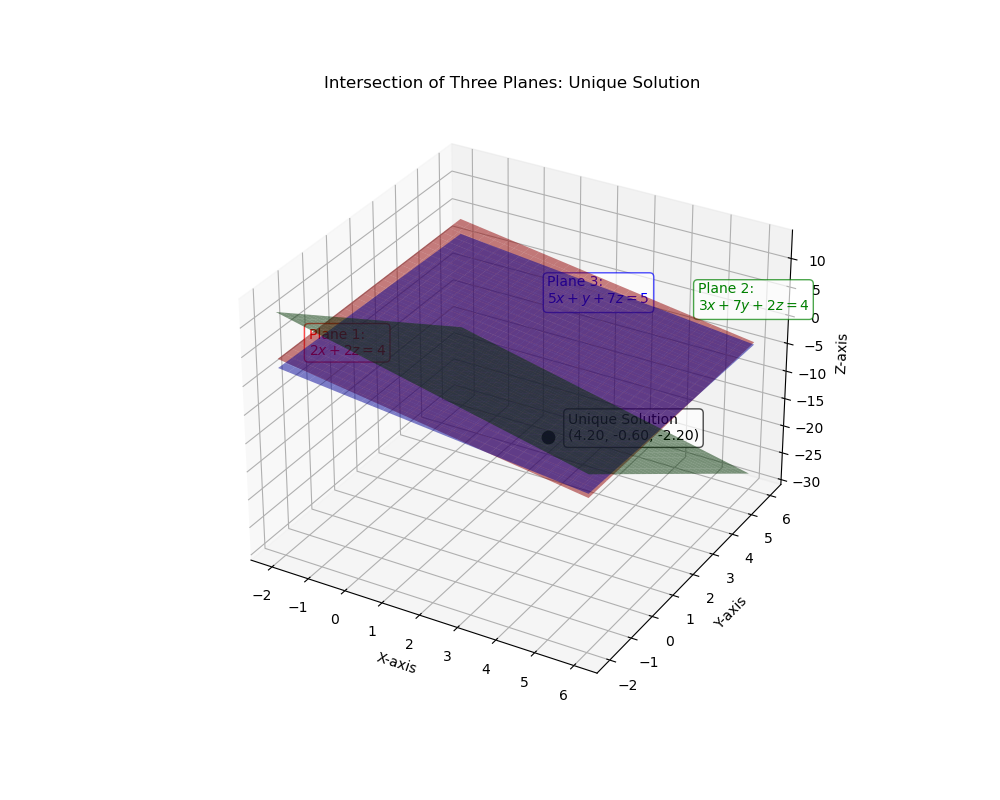
\includegraphics[width=\columnwidth, height=0.8\textheight, keepaspectratio]{Figure_23.png} 
\end{frame}
\end{document}
